
%(BEGIN_QUESTION)
% Copyright 2014, Tony R. Kuphaldt, released under the Creative Commons Attribution License (v 1.0)
% This means you may do almost anything with this work of mine, so long as you give me proper credit

Testledninger for DC-voltmetre er vanligvis to separate ledere som forbinder instrumentet med et par prober. For svært følsomme instrumenter brukes ofte en spesiell tolederkabel kalt {\it koaksialkabel} i stedet for to separate ledninger. Koaksialkabel -- der en senterleder er ``skjermet'' av ytre flette eller folie som fungerer som den andre lederen -- har svært god immunitet mot indusert ``støy'' fra elektriske og magnetiske felt:

$$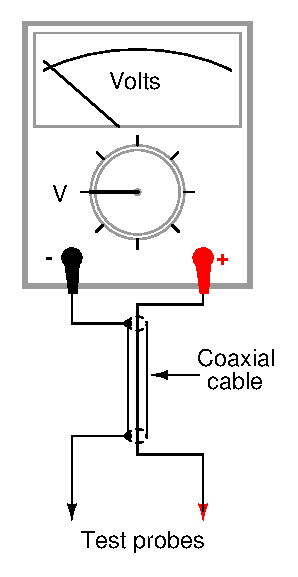
\includegraphics[width=5.5cm]{i00844x01.eps}$$

\filbreak

Ved måling av høyfrekvente AC-spenninger kan imidlertid parasittisk kapasitans og induktans i koaksialkabelen skape problemer. Vi kan representere disse fordelte kabel-egenskapene som ``lumpede'' parametere: én kondensator og én induktor som modellerer kabelens oppførsel:

$$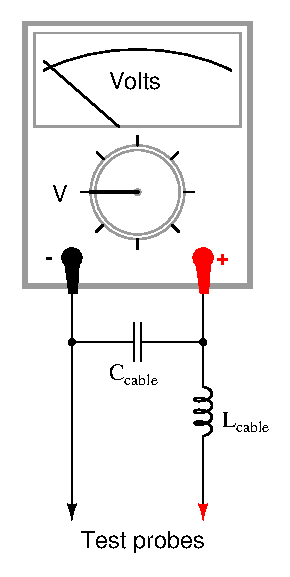
\includegraphics[width=5.5cm]{i00844x02.eps}$$

Typiske parasittverdier for en 10-fots kabel er 260 pF kapasitans og 650 $\mu$H induktans. Voltmeteret har selvfølgelig også egne iboende impedanser. I dette eksemplet antar vi at meterets ``input impedance'' er en enkel resistans på 1 M$\Omega$.

Beregn hvilken spenning meteret vil vise ved måling av en 20 V AC-kilde ved følgende frekvenser:

\begin{itemize}
\item{} $f =$ 1 Hz ; $V_{meter} =$
\item{} $f =$ 1 kHz ; $V_{meter} =$
\item{} $f =$ 10 kHz ; $V_{meter} =$
\item{} $f =$ 100 kHz ; $V_{meter} =$
\item{} $f =$ 1 MHz ; $V_{meter} =$
\end{itemize}

\underbar{file i00844}
%(END_QUESTION)





%(BEGIN_ANSWER)

Det er ikke nødvendig å uttrykke svarene i kompleks form, siden et analogt voltmeter ikke viser fasevinkelen på den målte spenningen:

\begin{itemize}
\item{} $f =$ 1 Hz ; $V_{meter} =$ 20 V
\item{} $f =$ 1 kHz ; $V_{meter} =$ 20 V
\item{} $f =$ 10 kHz ; $V_{meter} =$ 20.01 V
\item{} $f =$ 100 kHz ; $V_{meter} =$ 21.43 V
\item{} $f =$ 1 MHz ; $V_{meter} =$ 3.526 V
\end{itemize}

%(END_ANSWER)





%(BEGIN_NOTES)


%INDEX% Electronics review: AC reactance and impedance
%INDEX% Electronics review: series-parallel AC circuits

%(END_NOTES)
